\documentclass[conference]{IEEEtran}
\usepackage{amsmath,amssymb,booktabs,graphicx,microtype,url,xcolor}
\usepackage[hidelinks]{hyperref}
\hypersetup{pdftitle={Graph Conditional Flows for Sensor Fault Testing and Repair},pdfauthor={Alexander V. Mantzaris}}
\newcommand{\E}{\mathbb{E}}
\newcommand{\1}{\mathbf{1}}
\newcommand{\LME}{\operatorname{LME}}
\renewcommand{\theequation}{E\arabic{equation}}
% BEGIN GENERATED graph_flow/numbers.tex
\newcommand{\MacroRatioAP}{0.438}
\newcommand{\MacroPCAAP}{0.307}
\newcommand{\MacroNLLAP}{0.423}
\newcommand{\PCADifference}{0.131}
\newcommand{\NLLDifference}{0.015}
\newcommand{\PPCADifference}{0.054}
\newcommand{\TotalCases}{1,500}
\newcommand{\TotalCandidates}{54,080}
\newcommand{\AuditCandidates}{107,620}
\newcommand{\AuditMaximum}{$9.09\times10^{-13}$}
\newcommand{\PilotTime}{9.69}
\newcommand{\PilotInitial}{10.669}
\newcommand{\PilotFinal}{5.722}
\newcommand{\PilotInverse}{$7.15\times10^{-7}$}
\newcommand{\IntelEligibility}{65.0}
\newcommand{\IntelMisses}{37}
\newcommand{\ReplayDensity}{0}
\newcommand{\ReplayGeneration}{0}
\newcommand{\ReplayCorruption}{$9.12\times10^{-12}$}
\newcommand{\ReplayRatio}{$3.95\times10^{-12}$}
\newcommand{\ReplayPosterior}{$1.97\times10^{-12}$}
\newcommand{\ReplayJacobian}{$3.55\times10^{-15}$}
\newcommand{\ReplayBundles}{30}
% END GENERATED graph_flow/numbers.tex
\title{Graph Conditional Flows for Sensor Fault Testing and Repair}
\author{\IEEEauthorblockN{Alexander V. Mantzaris}
\IEEEauthorblockA{School of Data, Mathematical and Statistical Sciences\\University of Central Florida\\Orlando, FL, USA\\alexander.mantzaris@ucf.edu}}
\begin{document}
\maketitle
\begin{abstract}
An unusual sensor interval can reflect an incorrect measurement or a legitimate process change. We test fault localization with a neural normalizing flow conditioned on history and other physical sources through a predictive graph. GPU-generated reference intervals pass through normalized bias, drift, noise and stuck-reading channels. Integrating these possibilities gives a fault density whose ratio to the ordinary flow density supplies the detection score. Weighted generations provide conditional repairs. Comparators include PCA, the identical flow's likelihood, matched probabilistic PCA and the author GANF implementation. The fixed protocol covers a synthetic family, Intel Berkeley and SKAB, with sensor injections separate from native process events. % BEGIN GENERATED graph_flow/abstract_results.tex
The ratio improves the three-family mean AP by 0.131 over PCA and 0.015 over same-flow likelihood, with both paired primary intervals above zero. The latter misses the declared 0.02 usefulness margin. Neural benefit over matched PPCA and benefit from integration over a mean replacement remain inconclusive. Supervised trees perform better, and real-data alarm and repair failures limit operational claims.
% END GENERATED graph_flow/abstract_results.tex
 Versioned graph evidence and a sensor network view expose useful explanations and failures.
\end{abstract}
\begin{IEEEkeywords}
sensor data quality, conditional generation, fault localization, likelihood ratio, repair uncertainty
\end{IEEEkeywords}

\section{Introduction}
Distributed sensing connects physical measurements to digital twins and shared data spaces. Surprise alone does not identify a broken sensor. A coordinated physical change can be rare while every sensor reports it correctly. A stuck interval can be wrong without having an extreme value. Operators need evidence about named measurements and proposed changes.

The normal explanation treats the recorded interval as a conditional model draw. The fault explanation generates an uncorrupted interval and passes it through a measurement corruption channel. Integrating over plausible references gives a likelihood ratio and weighted repair distribution. Supporting sensors are conditioning information, not independent withheld witnesses. Predictive edges do not establish causation.

Our primary hypothesis H1 is that this integrated score improves sensor-interval average precision over both a development-selected PCA detector and ordinary negative log likelihood from the identical flow. H2 asks whether a flexible neural distribution improves on conditional Gaussian or probabilistic PCA models using the same corruption channels. H3 asks whether a separately selected recommendation policy increases useful repair coverage at a controlled failure rate. H3 is secondary and cannot replace an unsupported detection claim.

The contribution is an audited empirical procedure with tests of inaccessible targets, mismatched faults and corrupted context. The earlier diffusion witness study is preserved and rerun on shared cases. Fresh synthetic trajectories provide new simulator tests. Previously examined real partitions provide prospective injection tests, not untouched field validation.

\section{Related Work}
PCA residuals are established monitoring tools~\cite{pca}. Probabilistic PCA and its mixture extension supply normalized distributions, generation and uncertainty~\cite{ppca,mppca}. Neural benefits must therefore be measured against these probabilistic repair alternatives.

GANF combines recurrence, learned graphs and flows for anomaly detection~\cite{ganf}. MTGFlow studies dynamic graphs and entity-specific densities~\cite{mtgflow}. Recent work examines departures in conditional-flow latent dynamics~\cite{latentflow}. We use unchanged author GANF classes with documented evaluation adapters. Our affine couplings follow established constructions~\cite{realnvp}. Neither graph conditioning nor invertibility is new here.

Likelihood ratios for distributional anomalies have substantial precedent~\cite{ratio}. Bayesian sensor diagnosis predates neural flows~\cite{bayesfault}, and particle filtering integrates uncertain latent system states when assessing sensor fault explanations~\cite{wright}. A flow prior combined with a structured noise likelihood has also been used for inverse recovery~\cite{whang}. These are close conceptual predecessors. Our study evaluates a particular combination of masked graph context, normalized short-block corruption channels, marginal likelihood comparison and weighted repair. We do not claim invention of likelihood ratios or Bayes' rule.

CSDI and PriSTI generate conditional imputations~\cite{csdi,pristi}. ImDiffusion uses diffusion imputation for anomaly detection~\cite{imdiffusion}, and GDN uses graph-based forecast deviations~\cite{gdn}. We retain GDN and documented diffusion comparators. Our earlier procedure tested repairs against excluded witness measurements. The present conditional likelihood method does not inherit that independence claim. A source comparison matrix records implementation differences.

\section{Conditional Fault Explanations}
\subsection{Candidate population and allowed information}
A candidate $h$ names one channel and its final eight completed observations in a 64-step window. The window stride is 32. Let $y_h\in\mathbb R^{D_h}$ be the recorded target block and $z_h$ a possible uncorrupted noisy measurement. The primary implementation requires all $D_h=8$ target values. An unavailable target receives an availability flag and a common ranking floor, so excluded faults remain misses. It is never filled with zero and evaluated as a complete density.

Training medians and interquartile scales normalize each channel. Missing context has an explicit mask. We remove the candidate source's target interval from all channels belonging to that physical source before computing temporal features, lagged inputs or graph messages. Earlier observations of that source remain allowed. Known copies of the same measurement are canonicalized before input construction. Tests alter hidden values and aliases while holding latent draws fixed. The context and generated prior must remain unchanged, although the evaluated target density should change.

The frozen graph $G$ contains predictive associations selected using training and development data. Each edge stores direction, lag, units, training correlation and development support. The encoder uses up to three incoming channels from distinct other source groups, a shared gated recurrent unit, source embeddings and a masked mean of graph messages. Its context vector is $c_h=\operatorname{Encoder}_{\psi}(C_h,G)$. All data are available by the decision timestamp. Graph lags and recurrent steps count observations. They do not claim equal elapsed time in irregular recordings.

\subsection{Neural density and actual generation}
An invertible conditional flow maps a target block to a standard normal latent vector. With $f_\theta$ denoting the forward map,
\begin{equation}
 \log p_\theta(y_h\mid c_h)=\log p_0(f_\theta(y_h;c_h))
 +\log\left|\det\frac{\partial f_\theta}{\partial y_h}\right|.
\end{equation}
The conditioner is fixed when this target Jacobian is evaluated. Alternating affine couplings have triangular Jacobians and bounded neural log scales. A conditional location and scale transform precedes them. Generation applies the inverse on the GPU,
\begin{equation}
 \epsilon_h^{(m)}\sim\mathcal N(0,I),\qquad
 z_h^{(m)}=f_\theta^{-1}(\epsilon_h^{(m)};c_h).
\end{equation}
These are numerical sensor trajectories. They enter both the fault score and the repair calculation below. The reference training objective is
\begin{equation}
 \mathcal L_{\rm density}=-\frac{1}{N}\sum_{h=1}^{N}\log p_\theta(y_h\mid c_h).
\end{equation}
Reference denotes the declared training population, not certified healthy instrumentation. Saved records contain masks, contexts, latent draws, generated intervals and model hashes for representative production cases.

\begin{figure*}[!t]
 \centering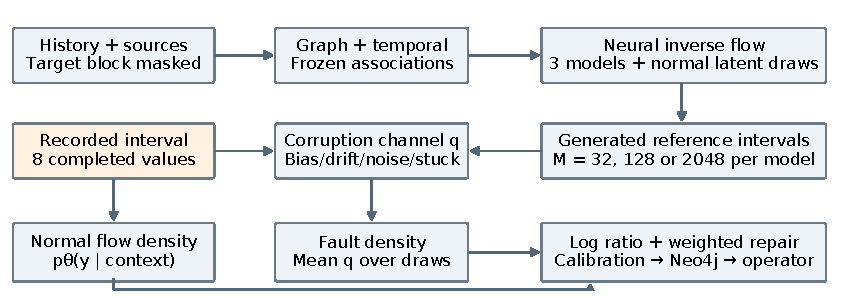
\includegraphics[width=\textwidth]{figures/graph_flow/architecture.pdf}
 \caption{Executed dataflow. The recorded target reaches density and corruption evaluation but is removed from the generation context. Generated trajectories directly enter the marginal fault density and the weighted repair. Graph persistence stores evidence references after numerical scoring.}
 \label{fig:architecture}
\end{figure*}

\subsection{Normalized corruption channels}
The normal explanation uses the flow density directly,
\begin{equation}
 p_{{\rm normal},h}(y_h\mid C_h,G)=p_\theta(y_h\mid c_h).
\end{equation}
The fault explanation uses a normalized mixture
\begin{equation}
 q_\phi(y\mid z)=\sum_{k=1}^{4}\pi_k\mathcal N(y;H_kz,R_k),
 \qquad \pi_k=\tfrac14.
\end{equation}
For bias, drift and excess noise, $H_k=I$. For a stuck reading, $H_k=\1 e_1^T$, so the uncertain stuck level is centered on the first generated reference value. Let $s\in\{1,2\}$ be the development-selected scale and $r=0.25$ the fixed noise floor. The covariances are
\[
\begin{split}
 R_{\rm bias}&=s^2\1\1^T+r^2I,\qquad
 R_{\rm drift}=s^2tt^T+r^2I,\\
 R_{\rm noise}&=s^2I,\qquad
 R_{\rm stuck}=s^2\1\1^T+r^2I.
\end{split}
\]
Here $t$ is the actual target timestamp ramp rescaled to $[-1,1]$. Bias and drift amplitudes are shared across the block. Independent amplitudes at every coordinate would be different models. Positive floors make each covariance positive definite. Cholesky-based determinants and quadratic forms give valid Gaussian densities. Dropout is an availability event and is not represented by a numeric corruption density.

The marginal fault density and log ratio are
\begin{align}
 p_{{\rm fault},h}(y_h\mid c_h)&=\int q_\phi(y_h\mid z)p_\theta(z\mid c_h)\,dz, \\
 S_h&=\log p_{{\rm fault},h}(y_h\mid c_h)-\log p_\theta(y_h\mid c_h).
\end{align}
Positive $S_h$ favors the declared fault model. It is not itself a calibrated probability or proof of sensor failure. With generated trajectories from (E2),
\begin{equation}
 \widehat S_h=\log\left[\frac{1}{M}\sum_{m=1}^{M}q_\phi(y_h\mid z_h^{(m)})\right]
 -\log p_\theta(y_h\mid c_h).
\end{equation}
We use stable log-sum-exp arithmetic. The logarithm of the average density is essential. Averaging log densities or taking the best generation does not implement this integral. The density estimate is unbiased under independent prior sampling, but its logarithm generally has downward bias.

For $E$ equally weighted trained models with $M$ samples each,
\begin{equation}
\begin{split}
 \widehat S_{h,E}={}&\LME_{e,m}\bigl[\log q_\phi(y_h\mid z_h^{(e,m)})\bigr]\\
 &-\LME_e\bigl[\log p_{\theta_e}(y_h\mid c_h)\bigr],
\end{split}
\end{equation}
where $\LME(a_1,\ldots,a_n)=\log(\sum_i\exp(a_i)/n)$. The ordinary-flow comparator is the negative second term's underlying mixture log density, using exactly the same checkpoints. An average of member log ratios is a separately labeled ablation.

\subsection{Repair distribution and numerical adequacy}
Bayes' rule under the fault explanation gives
\begin{equation}
 p(z\mid y_h,c_h,H_{1,h})=
 \frac{q_\phi(y_h\mid z)p_\theta(z\mid c_h)}{p_{{\rm fault},h}(y_h\mid c_h)}.
\end{equation}
For a uniform ensemble, we normalize $q_\phi(y_h\mid z_h^{(e,m)})$ over all generated members and samples to obtain weights $w_{e,m}$. Weighted means evaluate squared-error repair, and weighted medians and marginal quantiles are also retained. The reference truth never chooses a sample. A mean need not preserve a physical mode.
\begin{equation}
 \operatorname{ESS}_h=\left(\sum_{e,m}w_{e,m}^2\right)^{-1}.
\end{equation}
An ESS below 16 prevents a repair recommendation but leaves the detection score in the evaluated population. Low ESS identifies poor importance-sampling resolution, not necessarily large physical uncertainty. Repeated sampling seeds and a finite draw grid diagnose this limitation separately from differences between trained models.

We apply a proposed action to the full evaluated window. With normalized squared loss $L$ summed over observed cells and divided by eight, reference $y_j^\star$, acceptance $a_j$ and useful-improvement threshold $\delta=0.01$,
\begin{equation}
\begin{split}
 \Delta_j&=L(y_j,y_j^\star)-L(\operatorname{repair}_j,y_j^\star),\\
 F_j&=\1\{\text{wrong target}\ \text{or}\ \Delta_j\leq\delta\},\\
 \operatorname{Coverage}&=\frac{\sum_j a_j}{n},\quad
 \operatorname{Risk}=\frac{\sum_j a_jF_j}{\sum_j a_j}.
\end{split}
\end{equation}
A wrong-target action includes damage to previously correct measurements. Harmful edits have $\Delta_j<0$. No accepted action gives zero coverage and undefined risk. On real datasets the repair reference is the pre-injection recording, not unknown physical truth.

\section{Mathematical Checks and Limits}
\subsection{Normalization and the ideal ratio}
For fixed context, both the flow and every corruption channel are normalized on the same continuous target space. Nonnegativity permits exchanging integrals in (E6). Integrating first over $y$ yields $\int p_\theta(z\mid c)\,dz=1$. Thus the fault explanation is a normalized density. Quantized readings use a consistent continuous approximation for both explanations.

If the true healthy conditional law is exactly $p_{\rm normal}$ and $p_{\rm fault}$ is absolutely continuous with respect to it, then
\[
 \E_{H_0}[\exp(S_h)\mid c_h]=\int p_{\rm fault}(y\mid c_h)\,dy=1.
\]
Markov's inequality implies $\Pr_{H_0}(S_h\geq\log(1/\alpha)\mid c_h)\leq\alpha$. This is an established likelihood-ratio consequence. Density error, context contamination and distribution shift can invalidate its use for a fitted detector. A maximum across candidates does not inherit this single-candidate bound. A fixed convex mixture of valid ratios retains the ideal expectation property by linearity, but weights selected from the tested observation need separate justification. Our operational alarms therefore calibrate the actual maximum over all candidates.

\subsection{Gaussian reference and units}
For $z\sim\mathcal N(\mu,\Sigma)$ and $y=z+\eta$ with independent $\eta\sim\mathcal N(0,R)$, Gaussian convolution gives $p_{\rm fault}(y)=\mathcal N(y;\mu,\Sigma+R)$. Subtracting normal log densities gives
\[
 S=-\tfrac12\log\frac{|\Sigma+R|}{|\Sigma|}
 +\tfrac12(y-\mu)^T[\Sigma^{-1}-(\Sigma+R)^{-1}](y-\mu).
\]
Completing the square gives repair mean $\mu+\Sigma(\Sigma+R)^{-1}(y-\mu)$ and covariance $\Sigma-\Sigma(\Sigma+R)^{-1}\Sigma$. Replacing $z$ by $H_kz$ extends the formula to every channel in (E5). Conditional PPCA uses these exact integrations and mixture posterior weights. It therefore tests the same fault knowledge without neural Monte Carlo integration.

For a common invertible coordinate change $u=g(y)$, consistently transformed normal and fault densities both acquire $|\det Dg^{-1}(u)|$. Their ratio is unchanged. This is a statement about transforming the same two distributions, not retraining on arbitrary scales or changing the corruption prior. Numerical tests include a non-diagonal affine change of units.

\subsection{Identifiability}
Consider two sensors reporting a common process $x_t$. A genuine change to $x_t+a_t$ gives observations $(x_t+a_t,x_t+a_t)$. An unchanged process with additive failure $a_t$ in both sensors gives the identical observations. No function of these measurements can distinguish the explanations without further information. The stress study constructs and stores such paired observations and distinct latent truth. The ambiguity label denotes this known counterexample. It does not claim that the detector recognizes every ambiguous situation.

\section{Experimental Protocol}
\subsection{Datasets, independence and candidates}
Table~\ref{tab:data} gives the complete final candidate population. S32L, S32N and S64N are linear 32-channel, nonlinear 32-channel and nonlinear 64-channel configurations of one coupled synthetic family. They share a simulator design and are not counted as independent datasets. New final trajectories separate latent process state, uncorrupted noisy measurements and injected corruption. The last two of twelve final trajectories use the predeclared operating-regime shift. The linear setting is retained.

Intel contains 48 channels from twelve physical motes with temperature, humidity, light and voltage measurements~\cite{intel}. Completed five-minute bins preserve availability without interpolation. Chronological splits and gaps remain unchanged. SKAB retains eight sensor/process channels and experiment-level splits~\cite{skab}. Native process-event labels remain a separate task. Only reference windows without native events supply controlled fault cases. Training-only scaling and physical-source groups are reused throughout.

Every real partition had informed the preceding study. New injections do not establish transfer to untouched environments. No test observation moves into training. Synthetic training, development and calibration retain earlier sources so the legacy comparator has the same training opportunity.

We sample reference windows by source block, then create one unchanged copy and four fault copies. Development and calibration use bias, drift, excess noise and stuck readings. Each final reference has two known-family faults and two held-out-family faults, rotating across spike, scale, replay and delay. Final severities are new draws from the frozen range. Candidate labels require an actual change in an observed target coordinate. Wholly unobservable injection attempts remain availability outcomes. Other physical sources are unchanged by primary injections. This does not certify that real supporting recordings are physically fault-free.

% BEGIN GENERATED graph_flow/data_table.tex
\begin{table*}[t]
\centering
\caption{Evaluated populations. Blocks show training and final source blocks. Eligibility is complete availability of the eight target observations. Missing targets remain in the primary population.}
\label{tab:data}
\small
\begin{tabular}{lrrrrrr}
\toprule
Config. & $C$ & Blocks & Cases & Candidates & Faults & Eligible \\
\midrule
S32L & 32 & 12/12 & 320 & 10,240 & 256 & 100.0\% \\
S32N & 32 & 12/12 & 320 & 10,240 & 256 & 100.0\% \\
S64N & 64 & 12/12 & 320 & 20,480 & 256 & 100.0\% \\
Intel & 48 & 14/6 & 220 & 10,560 & 138 & 65.0\% \\
SKAB & 8 & 7/10 & 320 & 2,560 & 255 & 100.0\% \\
\bottomrule
\end{tabular}
\end{table*}
% END GENERATED graph_flow/data_table.tex

\subsection{Development selection and comparators}
The flow grid crosses two width/layer pairs, $(32,4)$ and $(64,6)$, with context lengths 32 and 56. Each fit uses 600 AdamW steps, batches of 128, learning rate 0.001 and weight decay 0.0001. Normal development likelihood selects checkpoints and capacity. Three fixed seeds form one density-mixture ensemble, not three ensemble repetitions. S32N and SKAB learning curves use one quarter, one half and all training blocks. Table~\ref{tab:runtime} gives model and training sizes.

Development also selects between corruption scales 1 and 2. The draw grid is $M\in\{32,128,512,2048\}$. We choose the smallest budget whose 95th percentile absolute score difference from the 2048-draw reference is at most 0.25 and rank correlation is at least 0.98, or use the maximum if no smaller budget passes. These are finite numerical diagnostics, not exact-integration guarantees. Separate sampling seeds test repeatability. All choices, data hashes and numerical source hashes are locked before final scoring.

PCA retains current and four-lag reconstruction with ranks 2, 4, 8 and 16 where valid. Development candidate AP selects the model. Its score averages current-channel squared reconstruction residual over the same eight-step target. Window maxima and the conventional full residual norm remain separately stored. Conditional PPCA and two-component mixture PPCA use ranks 2, 4 or 8 selected by normal development likelihood. They condition on the same graph-restricted observations and apply exactly the same $q_\phi$. An all-channel PPCA variant is named separately. Missing context is marginalized during conditional evaluation. Training context is mean-filled for parameter estimation, which is a limitation when missingness is informative.

The GANF comparison imports the authors' unchanged recurrent, graph and autoregressive-flow classes at a pinned revision. Widths 16 and 32, ten outer graph-optimization iterations and forty steps per iteration form its bounded grid. The adapter excludes missing target losses and same-source adjacency, and aggregates the final eight coordinate densities. GANF can use preceding target observations inside that interval and fills missing context for its original architecture without a mask input. Finite graph optimization can leave a nonzero acyclicity residual. We report it rather than claiming exact convergence. MTGFlow was inspected but not executed within the fixed budget.

A modest gradient-boosted classifier receives shape, earlier history, PCA residual and availability features. It is trained on the same four development fault mechanisms injected into training windows. This tests whether explicit fault information alone explains gains. The old diffusion witness, GDN, backbone residual and documented DiffAD adaptation are rerun on the shared manifests. The witness method retains its top-four screen. Excluded candidates receive a floor and true faults remain misses. Its old window-level results remain separately archived.

\subsection{Confidence and decision policy}
Whole calibration source blocks have three disjoint roles. Labeled blocks fit a logistic probability calibration using a robustly scaled score and scorable indicator, with the same opportunity for every comparator. Separate normal blocks calibrate the maximum score over the actual candidate procedure. If there are $n$ normal calibration windows,
\[
 p_{\rm window}=\frac{1+\sum_{b=1}^{n}\1\{S_{\max,b}\geq S_{\max,{\rm new}}\}}{n+1}.
\]
The minimum value is $1/(n+1)$. Small calibration populations cannot support arbitrary nominal false-alarm levels. Dependence and shift also limit guarantees.

The remaining calibration blocks select a repair probability threshold from a fixed grid. We maximize coverage subject to at least ten actions and a one-sided 95\% Wilson failure upper bound at most 0.10. If no threshold qualifies, the policy abstains. This bound is a calibration diagnostic under dependent data, not a guaranteed deployment risk. Actual test failure and harm remain reported. Marginal CRPS, interval coverage and width, and a joint energy score assess distributions~\cite{crps}. The flow energy estimate uses 512 weighted sample pairs.

\subsection{Endpoints and uncertainty}
Primary AP pools all sensor intervals, including clean windows and uncorrupted candidates. We never average AP only over windows containing a fault. For comparator $b$, the registered contrast is
\[
 \Delta_b=\tfrac13\sum_{d\in\{\mathrm{synthetic,Intel,SKAB}\}}
       (\operatorname{AP}_{\rm ratio,d}-\operatorname{AP}_{b,d}),
\]
averaging the three synthetic configurations within their family first. A chosen usefulness margin is 0.02 absolute AP. Directional H1 requires positive evidence against both PCA and same-flow NLL.

We use 1000 paired whole-block bootstrap replicates. Synthetic trajectories, Intel time blocks and SKAB experiments are resampled, retaining all correlated candidates and injected copies. Paired 32-channel synthetic seeds share bootstrap draws. The two primary contrasts use 97.5\% individual intervals, yielding a Bonferroni simultaneous 95\% statement. Dataset intervals are descriptive. Few real source blocks limit their stability, and training seeds are not independent test subjects. Secondary metrics cover localization, window detection, calibration, review precision, repairs and actual costs.

\section{Results}
\subsection{Primary comparison and neural contribution}
% BEGIN GENERATED graph_flow/ap_table.tex
\begin{table*}[t]
\centering
\caption{Sensor-interval average precision over the full candidate population. The synthetic configurations form one family in the macro-average. All methods use identical cases and complete-target eligibility.}
\label{tab:ap}
\small
\begin{tabular}{lrrrrrr}
\toprule
Method & S32L & S32N & S64N & Intel & SKAB & Macro \\
\midrule
Flow + corruption & 0.589 & 0.633 & 0.608 & 0.075 & 0.628 & 0.438 \\
PCA residual & 0.680 & 0.659 & 0.541 & 0.018 & 0.275 & 0.307 \\
Same-flow NLL & 0.588 & 0.632 & 0.600 & 0.058 & 0.604 & 0.423 \\
Graph PPCA + corruption & 0.654 & 0.629 & 0.594 & 0.032 & 0.494 & 0.384 \\
Mixture PPCA + corruption & 0.654 & 0.626 & 0.584 & 0.028 & 0.473 & 0.374 \\
All-channel PPCA + corruption & 0.722 & 0.697 & 0.474 & 0.019 & 0.394 & 0.348 \\
Official GANF & 0.532 & 0.473 & 0.290 & 0.015 & 0.230 & 0.225 \\
Supervised trees & 0.708 & 0.700 & 0.641 & 0.366 & 0.686 & 0.578 \\
Legacy diffusion witness & 0.494 & 0.632 & 0.449 & 0.014 & 0.188 & 0.242 \\
GDN residual & 0.305 & 0.416 & 0.429 & 0.024 & 0.265 & 0.224 \\
Diffusion residual & 0.665 & 0.623 & 0.439 & 0.016 & 0.379 & 0.324 \\
DiffAD adaptation & 0.482 & 0.443 & 0.299 & 0.029 & 0.481 & 0.306 \\
\bottomrule
\end{tabular}
\end{table*}
% END GENERATED graph_flow/ap_table.tex
% BEGIN GENERATED graph_flow/primary_results.tex
The locked evaluation contains 1,500 cases and 54,080 candidate intervals. Family-macro AP is 0.438 for the ratio, 0.307 for PCA and 0.423 for same-flow NLL. The paired differences are +0.131 [+0.093, +0.147] against PCA and +0.015 [+0.005, +0.027] against NLL. Both simultaneous primary intervals are positive, supporting the directional H1 for this defined protocol. The NLL contrast is smaller than the chosen 0.02 practical margin.

This aggregate does not imply improvement in every environment. PCA is stronger on both 32-channel synthetic settings, with negative paired intervals for the ratio. The ratio improves on PCA in S64N and the two real families. SKAB contributes most of the macro difference. Intel remains weak in absolute terms despite its positive comparison. Only 65.0\% of Intel target blocks are eligible, and 37 changed targets remain unscorable misses.

The matched PPCA comparison is +0.054 [-0.007, +0.082]. Its interval spans zero, so H2 is inconclusive. The mixture-PPCA interval also spans zero. The conditional Gaussian control is particularly strong in the linear configuration. Supervised trees exceed the ratio in every configuration. Their macro advantage is 0.140, and the paired ratio-minus-tree interval is [-0.169, -0.114]. Thus the results do not establish the ratio as the strongest available detector when labeled injection mechanisms can be exploited. The author GANF and rerun legacy methods provide additional comparisons in Table~\ref{tab:ap}. Top-one ratio attribution is 0.660 on S32N, 0.065 on Intel and 0.631 on SKAB. Held-out mechanisms substantially reduce AP (Table~\ref{tab:strata}).
% END GENERATED graph_flow/primary_results.tex
\begin{figure*}[!t]
 \centering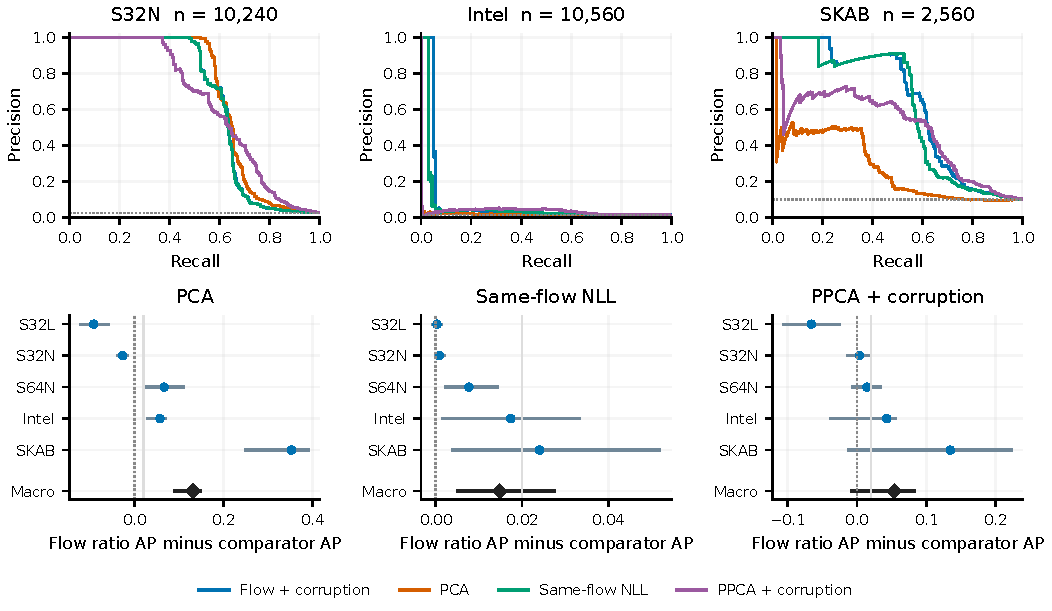
\includegraphics[width=\textwidth]{figures/graph_flow/performance.pdf}
 \caption{Sensor-interval precision--recall curves and paired AP differences. All configurations contribute to the three-family macro contrast. Dataset intervals are 95\%. The two primary macro intervals are 97.5\% individually.}
 \label{fig:performance}
\end{figure*}
% BEGIN GENERATED graph_flow/strata.tex
\begin{table}[t]
\centering
\caption{Known and held-out fault families, each pooled with clean windows. Entries give flow-ratio AP / PCA AP. Held-out mechanisms were absent from channel modeling and classifier development.}
\label{tab:strata}
\small
\begin{tabular}{lrr}
\toprule
Config. & Known & Held out \\
\midrule
S32L & 0.785/0.918 & 0.371/0.471 \\
S32N & 0.888/0.928 & 0.365/0.411 \\
S64N & 0.875/0.795 & 0.325/0.282 \\
Intel & 0.095/0.018 & 0.035/0.013 \\
SKAB & 0.790/0.318 & 0.420/0.208 \\
\bottomrule
\end{tabular}
\end{table}
% END GENERATED graph_flow/strata.tex

\subsection{Calibration, review and repair}
% BEGIN GENERATED graph_flow/confidence_results.tex
Confidence is not uniformly reliable. The ratio has lower Brier score than PCA in all synthetic configurations and SKAB, but a much worse Intel Brier score. Intel gives 0.068 with block interval [0.054, 0.082], compared with PCA's 0.017. Its smallest attainable window p-value is 0.059, so neither a 1\% nor a 5\% alarm level is representable. At level 0.10, 79 of 82 unchanged Intel cases alarm. The ratio's relative AP gain therefore does not establish a usable Intel alarm system. Normal cases include injection attempts that changed no observed coordinate.

The flow policy accepts useful synthetic repairs with no observed failures, but generally has lower coverage than PPCA. In S64N it accepts 125 of 320 cases, versus no PCA recommendation and 129 PPCA recommendations. Zero observed failures do not imply zero population risk, especially with dependent blocks. Intel accepts no repair and has undefined recommendation risk.

On SKAB the ratio accepts 123 repairs and makes 24 failed recommendations, all harmful. Actual risk is 0.195, with a wide block interval [0.000, 0.400], exceeding the calibration target in point estimate. PCA and PPCA risks are 0.371 and 0.183. H3 is not established as a general controlled-risk coverage advantage. Table~\ref{tab:repair} further shows that matched PPCA has lower repair CRPS and energy score in every configuration. Flow interval widths do not buy reliable real-data coverage. Figure~\ref{fig:repair} retains both successful and failed cases. Probability calibration concerns the designed injection prevalence, not operational physical-failure probabilities.
% END GENERATED graph_flow/confidence_results.tex
% BEGIN GENERATED graph_flow/confidence_table.tex
\begin{table*}[t]
\centering
\caption{Flow ratio confidence and selected repair policy on final cases. Alarms use the separately calibrated window maximum at level 0.10. Repair counts cover all evaluation cases. A dash denotes undefined risk because no action was accepted.}
\label{tab:confidence}
\small
\begin{tabular}{lrrrrrrrr}
\toprule
Config. & Brier & Log loss & Min. $p$ & False alarms & Recall & Repairs & Failed & Harmful \\
\midrule
S32L & 0.012 & 0.066 & 0.027 & 6/64 & 0.590 & 122 & 0/122 & 0 \\
S32N & 0.012 & 0.065 & 0.027 & 10/64 & 0.691 & 134 & 0/134 & 0 \\
S64N & 0.007 & 0.037 & 0.027 & 4/64 & 0.648 & 125 & 0/125 & 0 \\
Intel & 0.068 & 0.441 & 0.059 & 79/82 & 0.993 & 0 & -- & 0 \\
SKAB & 0.053 & 0.276 & 0.026 & 3/65 & 0.463 & 123 & 24/123 & 24 \\
\bottomrule
\end{tabular}
\end{table*}
% END GENERATED graph_flow/confidence_table.tex
% BEGIN GENERATED graph_flow/repair_table.tex
\begin{table}[t]
\centering
\caption{Oracle-target repair distributions on eligible injected faults. Width and scores use training-normalized measurement units. Interval coverage is measured for nominal 90\% marginal intervals. Lower CRPS and energy score are better.}
\label{tab:repair}
\small
\begin{tabular}{llrrrr}
\toprule
Config. & Prior & CRPS & Coverage & Width & Energy \\
\midrule
S32L & Flow & 0.157 & 0.930 & 1.328 & 0.468 \\
S32L & PPCA & 0.024 & 0.961 & 0.169 & 0.081 \\
S32N & Flow & 0.039 & 0.975 & 0.341 & 0.129 \\
S32N & PPCA & 0.027 & 0.909 & 0.167 & 0.092 \\
S64N & Flow & 0.084 & 0.912 & 0.488 & 0.285 \\
S64N & PPCA & 0.069 & 0.875 & 0.329 & 0.238 \\
Intel & Flow & 3.494 & 0.399 & 1.154 & 9.905 \\
Intel & PPCA & 0.827 & 0.344 & 0.232 & 2.454 \\
SKAB & Flow & 0.391 & 0.775 & 1.202 & 1.249 \\
SKAB & PPCA & 0.267 & 0.778 & 0.602 & 0.877 \\
\bottomrule
\end{tabular}
\end{table}
% END GENERATED graph_flow/repair_table.tex
\begin{figure*}[!t]
 \centering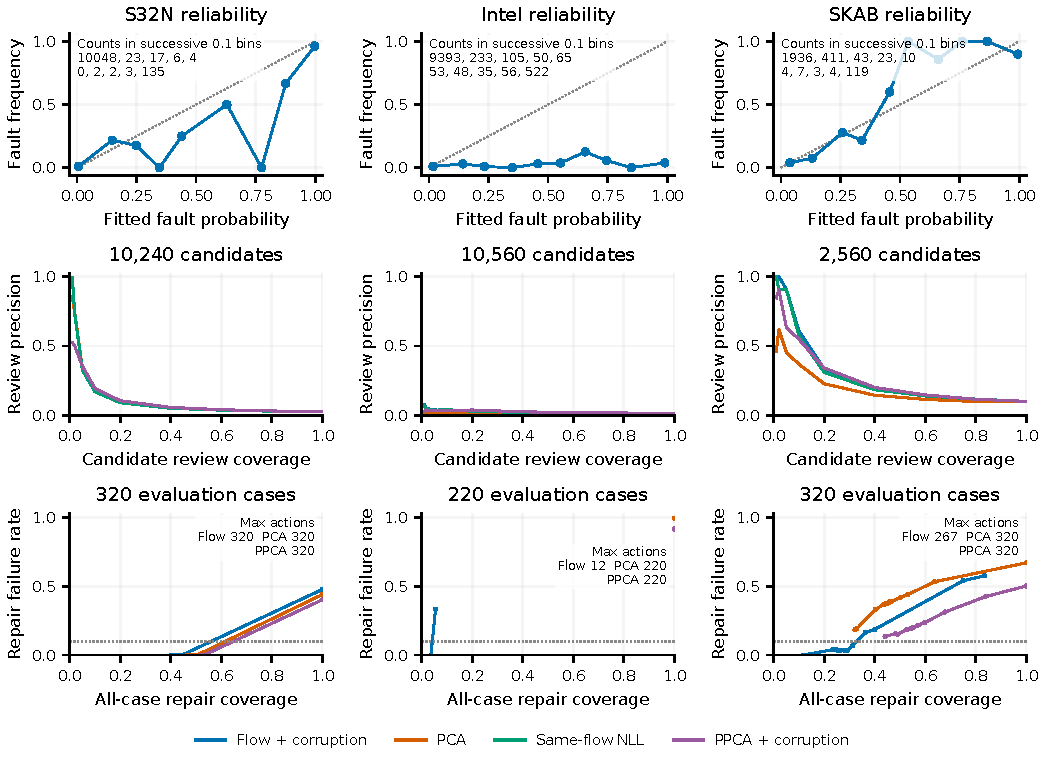
\includegraphics[width=\textwidth]{figures/graph_flow/confidence.pdf}
 \caption{Reliability, review precision and repair risk. Reliability insets count successive bins, five per line. Risk insets count actions at maximum coverage. Curves are threshold sweeps. Table~\ref{tab:confidence} gives calibration-selected actions. Zero coverage has undefined risk.}
 \label{fig:confidence}
\end{figure*}
\begin{figure*}[!t]
 \centering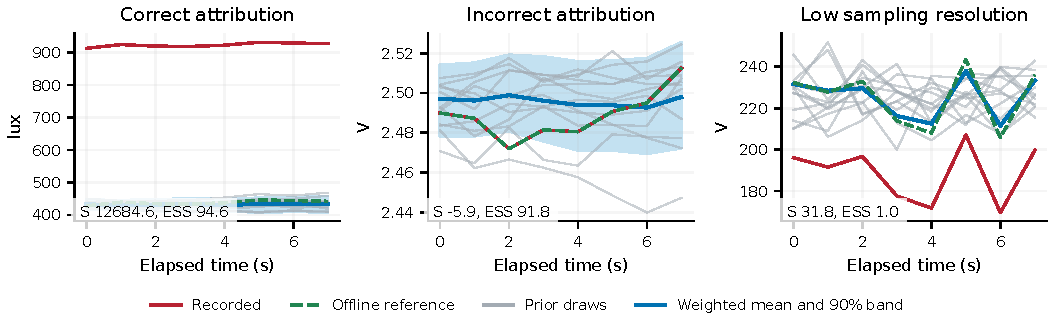
\includegraphics[width=\textwidth]{figures/graph_flow/repair.pdf}
 \caption{Cases chosen by frozen success, failure and numerical-adequacy rules. Gray trajectories are GPU generations. Blue bands are weighted 90\% marginal intervals. Reference truth is only for offline evaluation. Low ESS limits repair reliability. Case IDs and hashes are distributed with the figure.}
 \label{fig:repair}
\end{figure*}

\subsection{Ablations and adverse conditions}
% BEGIN GENERATED graph_flow/ablation_results.tex
Integrated generation improves macro AP over the prior-mean plug-in by 0.003, with interval [-0.007, +0.020]. This does not demonstrate that integration is needed for the measured detection gain. Graph context improves over own history by 0.053 [+0.028, +0.077]. Family-macro AP is 0.427 for a single member and 0.468 when member log ratios are averaged instead of mixing densities. All leave-one-corruption-channel-out results remain saved without selecting a new fault prior after testing. Scale sensitivity is retained from development.

Sampling error remains visible. At 2048 draws per member, the SKAB 95th percentile repeated-seed score change is 0.952. The maximum tested budget is a finite reference, not exact integration. Low-ESS cases remain detection outcomes and become recommendation abstentions. Missing support changes attribution in Table~\ref{tab:stress}. With multiple true faults, a lower original-target top-one rate alone does not mean an incorrect fault was chosen. For S32N with half the other sources corrupted, pooled AP over all true targets is 0.946, at the changed fault prevalence. Known-copy canonicalization gives exactly unchanged scores on every registered copy case.

The separate association diagnostic uses direct residuals. On the twelve S32N cases with half the graph associations changed, mean edge-localization AP is 0.977. Reading and association alarms can both fire or both remain silent. Their full cross-type counts are saved, and a reading ratio is never treated as proof that an edge is false. The synthetic physical-change counterexample produces identical observations for both explanations; 12 of 12 S32N physical-change cases trigger the reading alarm at 0.10. The separate native SKAB task contains 224 windows, including 78 process-event windows. Window AP is 0.536 for the ratio, 0.546 for NLL and 0.499 for PCA. These are process detections and do not validate sensor-fault diagnoses.
% END GENERATED graph_flow/ablation_results.tex
% BEGIN GENERATED graph_flow/stress_table.tex
\begin{table}[t]
\centering
\caption{Registered stress diagnostics on twelve source windows per configuration. First three columns give primary-target top-one rates. The last gives measurement alarms under a graph-only error affecting half the stored associations. This is cross-type confusion, not association diagnosis.}
\label{tab:stress}
\small
\begin{tabular}{lrrrr}
\toprule
Config. & Single & Half missing & Half faulty & Graph alarm \\
\midrule
S32L & 1.000 & 1.000 & 0.000 & 0.083 \\
S32N & 1.000 & 0.917 & 0.000 & 1.000 \\
S64N & 1.000 & 0.750 & 0.083 & 1.000 \\
Intel & 0.083 & 0.250 & 0.167 & 0.750 \\
SKAB & 0.833 & 0.750 & 0.167 & 0.250 \\
\bottomrule
\end{tabular}
\end{table}
% END GENERATED graph_flow/stress_table.tex
\begin{figure*}[!t]
 \centering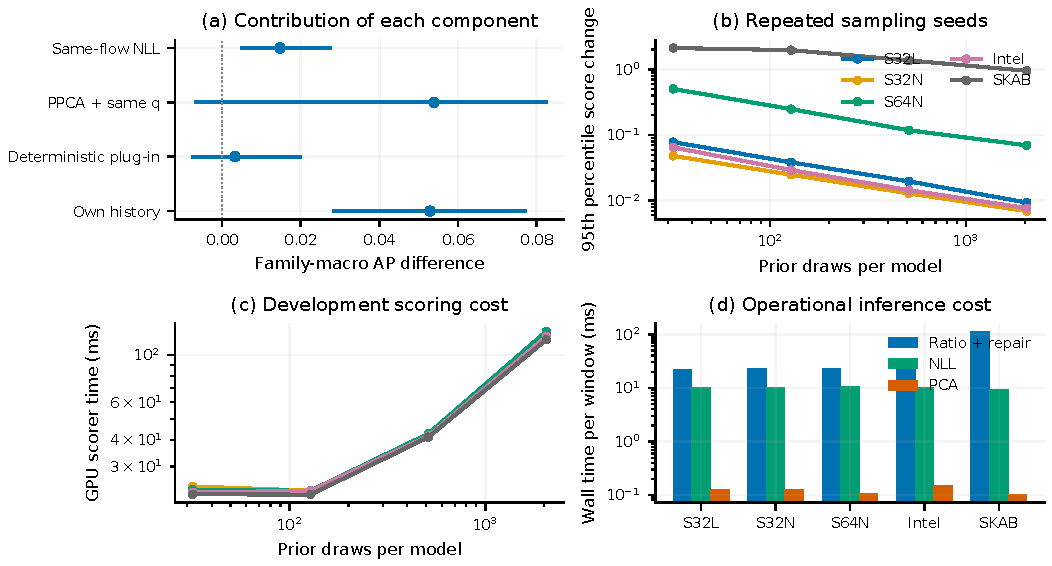
\includegraphics[width=\textwidth]{figures/graph_flow/equations.pdf}
 \caption{Equation contributions and computational costs. The plug-in replaces integration by the generated prior mean. Repeated seeds use fixed development cases. Panel (c) includes offline distribution metrics. Panel (d) measures operational scoring and repair without truth-dependent metrics.}
 \label{fig:equations}
\end{figure*}

\subsection{Numerical evidence and computation}
The scalar reference passes eight check groups. Forty local tests include eighteen flow checks covering inverse/Jacobian agreement, Gaussian integrals and posteriors, normalized corruption, units, stable mixture arithmetic, masking, missingness, source copies, chunking and repair damage. A Gaussian simulator trained a 22,048-parameter flow on the GPU. Validation NLL changed from \PilotInitial{} to \PilotFinal{} in \PilotTime{} seconds. This verifies computation, not benchmark superiority.

Production auditing recomputes \AuditCandidates{} calibration and final candidate scores from saved component integrals, with maximum discrepancy \AuditMaximum. Independently evaluated NumPy corruption densities and GPU model/draw replay cover \ReplayBundles{} full generation bundles. Maximum generation, normal-density, corruption-density and ratio discrepancies are \ReplayGeneration, \ReplayDensity, \ReplayCorruption{} and \ReplayRatio, respectively. Weighted posterior means agree within \ReplayPosterior. An autograd determinant from a trained model agrees with its analytic determinant within \ReplayJacobian. These checks establish implementation agreement, not adequacy of the fitted real-world distributions.

% BEGIN GENERATED graph_flow/runtime_table.tex
\begin{table}[t]
\centering
\caption{Selected model size, training intervals and operational latency on the RTX PRO 4500. Times are medians of seven warm full-window calls including repair summaries. Loading and offline truth metrics are excluded.}
\label{tab:runtime}
\small
\begin{tabular}{lrrrr}
\toprule
Config. & Params (k) & Train $N$ & $M$ & Ratio (ms) \\
\midrule
S32L & 96.9 & 11904 & 32 & 22.3 \\
S32N & 96.9 & 11904 & 32 & 22.7 \\
S64N & 97.4 & 23808 & 128 & 23.0 \\
Intel & 97.2 & 5072 & 32 & 22.5 \\
SKAB & 96.5 & 3272 & 2048 & 112.5 \\
\bottomrule
\end{tabular}
\end{table}
% END GENERATED graph_flow/runtime_table.tex
% BEGIN GENERATED graph_flow/runtime_results.tex
The bounded study completed 70 distinct neural fits including the Gaussian pilot. Their recorded fitting time sums to 10.8 minutes, excluding data preparation, Gaussian fitting, scoring and evaluation. The selected flows have 96,512 to 97,408 parameters per member. Peak allocation over the registered neural fits is 0.49 GiB. Selected GANF acyclicity residuals range from 1.53e-05 to 0.00776, documenting incomplete graph convergence within the finite budget. Training the selected three flow members takes 34.5 to 36.9 seconds per configuration. Same-flow NLL takes 9.3 to 10.5 milliseconds per window, compared with 0.10 to 0.15 for PCA. Table~\ref{tab:runtime} reports isolated operational wall times, including conditional repair summaries and returned evidence transfer. PCA and PPCA execute on the CPU. Float32 neural computation and float64 score arithmetic are used without mixed precision. The initial independent replay mistakenly retained float32 in a SciPy ensemble reduction. Explicit promotion corrected that audit without changing predictions, models or the protocol lock. The failed audit and correction are preserved.
% END GENERATED graph_flow/runtime_results.tex

\section{Graph Evidence and Operator Review}
Versioned Neo4j records link sensors, physical sources, windows, associations, models, fault hypotheses, generations, scores and repairs. Large arrays are content-addressed files. Original observations remain immutable. Accept, reject and defer decisions are separate records and do not apply repairs automatically.

The conventional two-dimensional network names sensors and annotates directed edges with lag and training correlation. Red outlines mark disputed intervals and blue outlines mark supporting sources. Amber dashed edges denote separately assessed association disputes. Details show observed and generated trajectories, weighted repair intervals, ESS, benchmark probability and abstention. Reading scores do not imply per-edge certainty.

\begin{figure}[!t]
 \centering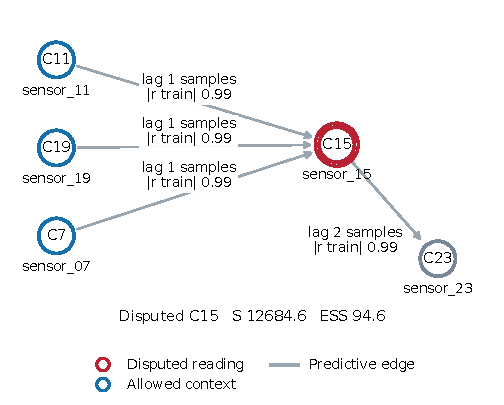
\includegraphics[width=\columnwidth]{figures/graph_flow/network.pdf}
 \caption{Saved S32N sensor network case with a topology-selected neighborhood. Gray arrows denote predictive associations, blue outlines mark conditioning sources, and red marks the disputed interval. Its score does not certify individual edges.}
 \label{fig:network}
\end{figure}
% BEGIN GENERATED graph_flow/interface_results.tex
The saved interface collection contains 23 cases, including first correct and incorrect attributions, inadequate sampling, constructed ambiguity and separate association review. Repeated Neo4j export leaves entity counts unchanged. Automated browser checks exercise evidence loading, node and edge selection, actual generated curves, hidden-by-default evaluation truth, artifact download, accept/reject/defer persistence and preservation of the observation. These checks are interface verification, not a human operator experiment.
% END GENERATED graph_flow/interface_results.tex

\section{Discussion and Limitations}
% BEGIN GENERATED graph_flow/discussion_results.tex
The positive primary contrast, driven mainly by SKAB, is narrower than a general neural-generation claim. The same-flow gain is small, and the PPCA and mean-plug-in controls leave its mechanism unresolved. Stronger supervised performance shows the value of explicit fault information outside a generative model. Repair and calibration are stricter tests than ranking alone. Intel abstention does not convert missed faults into successful detections, and SKAB repair risk exceeds the target in point estimate. The evidence supports further testing of operator review under declared assumptions.
% END GENERATED graph_flow/discussion_results.tex
The evaluated candidate is a short, complete, single-channel block. Primary injections affect one source at a time, with corrupted supporting sources studied separately. This is not a general multichannel failure model. Missing targets reduce population coverage substantially in Intel. Complete-target eligibility makes the density valid, but it does not solve observed-data flow inference. Quantization is approximated continuously, and temporal encoders do not fully represent irregular elapsed time.

The benchmark fault prevalence is determined by the injection design. Calibrated probabilities cannot be transported directly to operational failure prevalence or a mixture of physical and association events. Synthetic mechanisms and source blocks are limited, and the real test environments were previously examined. The finite architecture and comparator budgets do not establish the best attainable performance of any model family. Automated browser verification demonstrates interface behavior, not usefulness in a human operator study.

The previous window-level witness study remains recoverable and cannot be treated as independent confirmation. Reproduction bundles retain configuration locks, failed checks, score components and source hashes. Raw caches and model weights stay outside Git, with exact local and GPU locations documented. The paper can be rebuilt from distributed evidence without retraining.

\section{Conclusion}
% BEGIN GENERATED graph_flow/conclusion_results.tex
GPU-generated reference trajectories support an executable chain from normalized fault comparison to weighted repair and graph evidence. The frozen study supports directional H1 with a small score-specific gain. Neural necessity, integration benefit and controlled repair risk remain unestablished. Supervised performance, poor Intel confidence, held-out faults and context ambiguity define the next questions rather than being excluded from the evidence.
% END GENERATED graph_flow/conclusion_results.tex

% Bibliography embedded for a single-file LaTeX manuscript.
% Generated by IEEEtran.bst, version: 1.14 (2015/08/26)
\begin{thebibliography}{10}
\providecommand{\url}[1]{#1}
\csname url@samestyle\endcsname
\providecommand{\newblock}{\relax}
\providecommand{\bibinfo}[2]{#2}
\providecommand{\BIBentrySTDinterwordspacing}{\spaceskip=0pt\relax}
\providecommand{\BIBentryALTinterwordstretchfactor}{4}
\providecommand{\BIBentryALTinterwordspacing}{\spaceskip=\fontdimen2\font plus
\BIBentryALTinterwordstretchfactor\fontdimen3\font minus
  \fontdimen4\font\relax}
\providecommand{\BIBforeignlanguage}[2]{{%
\expandafter\ifx\csname l@#1\endcsname\relax
\typeout{** WARNING: IEEEtran.bst: No hyphenation pattern has been}%
\typeout{** loaded for the language `#1'. Using the pattern for}%
\typeout{** the default language instead.}%
\else
\language=\csname l@#1\endcsname
\fi
#2}}
\providecommand{\BIBdecl}{\relax}
\BIBdecl

\bibitem{pca}
J.~E. Jackson and G.~S. Mudholkar, ``Control procedures for residuals
  associated with principal component analysis,'' \emph{Technometrics},
  vol.~21, no.~3, pp. 341--349, 1979.

\bibitem{ppca}
M.~E. Tipping and C.~M. Bishop, ``Probabilistic principal component analysis,''
  \emph{Journal of the Royal Statistical Society, Series B}, vol.~61, no.~3,
  pp. 611--622, 1999.

\bibitem{mppca}
------, ``Mixtures of probabilistic principal component analysers,''
  \emph{Neural Computation}, vol.~11, no.~2, pp. 443--482, 1999.

\bibitem{ganf}
E.~Dai and J.~Chen, ``Graph-augmented normalizing flows for anomaly detection
  of multiple time series,'' in \emph{International Conference on Learning
  Representations}, 2022.

\bibitem{mtgflow}
\BIBentryALTinterwordspacing
Q.~Zhou, J.~Chen, H.~Liu, S.~He, and W.~Meng, ``Detecting multivariate time
  series anomalies with zero known label,'' 2023, arXiv:2208.02108v3. [Online].
  Available: \url{https://arxiv.org/abs/2208.02108}
\BIBentrySTDinterwordspacing

\bibitem{latentflow}
\BIBentryALTinterwordspacing
D.~Baumgartner, E.~de~Souza~da Silva, and I.~n. Urteaga, ``Anomaly detection in
  time-series via inductive biases in the latent space of conditional
  normalizing flows,'' in \emph{Uncertainty in Artificial Intelligence}, ser.
  Proceedings of Machine Learning Research, vol. 337, 2026, pp. 448--468.
  [Online]. Available:
  \url{https://proceedings.mlr.press/v337/baumgartner26a.html}
\BIBentrySTDinterwordspacing

\bibitem{realnvp}
L.~Dinh, J.~Sohl-Dickstein, and S.~Bengio, ``Density estimation using real
  {NVP},'' in \emph{International Conference on Learning Representations},
  2017.

\bibitem{ratio}
J.~Ren, P.~J. Liu, E.~Fertig, J.~Snoek, R.~Poplin, M.~A. DePristo, J.~V.
  Dillon, and B.~Lakshminarayanan, ``Likelihood ratios for out-of-distribution
  detection,'' in \emph{Advances in Neural Information Processing Systems},
  vol.~32, 2019.

\bibitem{bayesfault}
N.~Mehranbod, M.~Soroush, and C.~Panjapornpon, ``A method of sensor fault
  detection and identification,'' \emph{Journal of Process Control}, vol.~15,
  no.~3, pp. 321--339, 2005.

\bibitem{wright}
M.~A. Wright and R.~Horowitz, ``Particle-filter-enabled real-time sensor fault
  detection without a model of faults,'' in \emph{IEEE Conference on Decision
  and Control}, 2017.

\bibitem{whang}
\BIBentryALTinterwordspacing
J.~Whang, Q.~Lei, and A.~G. Dimakis, ``Solving inverse problems with a
  flow-based noise model,'' in \emph{International Conference on Machine
  Learning}, ser. Proceedings of Machine Learning Research, vol. 139, 2021.
  [Online]. Available: \url{https://proceedings.mlr.press/v139/whang21a.html}
\BIBentrySTDinterwordspacing

\bibitem{csdi}
\BIBentryALTinterwordspacing
Y.~Tashiro, J.~Song, Y.~Song, and S.~Ermon, ``{CSDI}: Conditional score-based
  diffusion models for probabilistic time series imputation,'' in
  \emph{Advances in Neural Information Processing Systems}, vol.~34, 2021.
  [Online]. Available:
  \url{https://proceedings.neurips.cc/paper/2021/hash/cfe8504bda37b575c70ee1a8276f3486-Abstract.html}
\BIBentrySTDinterwordspacing

\bibitem{pristi}
\BIBentryALTinterwordspacing
M.~Liu, H.~Huang, H.~Feng, L.~Sun, B.~Du, and Y.~Fu, ``{PriSTI}: A conditional
  diffusion framework for spatiotemporal imputation,'' 2023, arXiv:2302.09746.
  [Online]. Available: \url{https://arxiv.org/abs/2302.09746}
\BIBentrySTDinterwordspacing

\bibitem{imdiffusion}
\BIBentryALTinterwordspacing
Y.~Chen, C.~Zhang, M.~Ma, Y.~Liu, R.~Ding, B.~Li, S.~He, S.~Rajmohan, Q.~Lin,
  and D.~Zhang, ``{ImDiffusion}: Imputed diffusion models for multivariate time
  series anomaly detection,'' 2023, arXiv:2307.00754v2. [Online]. Available:
  \url{https://arxiv.org/abs/2307.00754}
\BIBentrySTDinterwordspacing

\bibitem{gdn}
A.~Deng and B.~Hooi, ``Graph neural network-based anomaly detection in
  multivariate time series,'' in \emph{Proceedings of the AAAI Conference on
  Artificial Intelligence}, vol.~35, no.~5, 2021, pp. 4027--4035.

\bibitem{intel}
{Intel Berkeley Research Lab}, ``Intel lab data,''
  \url{https://db.csail.mit.edu/labdata/labdata.html}, 2004, accessed September
  30, 2026.

\bibitem{skab}
\BIBentryALTinterwordspacing
I.~D. Katser and V.~O. Kozitsin, ``Skoltech anomaly benchmark ({SKAB}),'' 2020.
  [Online]. Available: \url{https://github.com/waico/SKAB}
\BIBentrySTDinterwordspacing

\bibitem{crps}
T.~Gneiting and A.~E. Raftery, ``Strictly proper scoring rules, prediction, and
  estimation,'' \emph{Journal of the American Statistical Association}, vol.
  102, no. 477, pp. 359--378, 2007.

\end{thebibliography}
\end{document}
